\documentclass[]{article} 


\usepackage{amsmath,amssymb,amsbsy,txfonts}
\usepackage{bbm,times}
\usepackage[T1]{fontenc}
\usepackage{braket}
\usepackage{epsfig} 

\usepackage{graphicx}% Include figure files
\usepackage{dcolumn}% Align table columns on decimal point
\usepackage{bm}% bold math
%\usepackage{ulem}

\usepackage{physics}
\usepackage{xcolor}

%\usepackage{hyperref}% add hypertext capabilities
%\usepackage{cleveref}
%\hypersetup{colorlinks=true, linkcolor=blue}

\usepackage{soul}
\usepackage{cancel}
\usepackage{float}
\usepackage{multirow}
\newcolumntype{?}{!{\vrule width 1.8pt}}

\usepackage{colortbl}

\graphicspath{{images/}}

% Custom commands
\renewcommand{\a}{\hat{a}}
\newcommand{\ad}{\hat{a}^\dagger}
\renewcommand{\b}{\hat{b}}
\newcommand{\bd}{\hat{b}^\dagger}
\newcommand{\opV}[1][k]{\hat{V}_{#1}}
\newcommand{\opU}[1][k]{\hat{U}_{#1}}
\newcommand{\ops}[2]{\hat{\sigma}_#1^#2}
\newcommand{\opsup}[1]{\dyad{e}{g#1}}
\newcommand{\opsdwn}[1]{\dyad{g#1}{e}}
\renewcommand{\tt}{\theta^2}
\newcommand{\dissipator}[1][n]{\mathcal{D}_S[\rho_{#1}]}
\newcommand{\ga}{\gamma_\alpha}
\newcommand{\gb}{\gamma_\beta}
\newcommand{\idd}{\mathbb{I}}
\newcommand{\C}{\hat{C}}
\newcommand{\Cp}{\hat{C}'}
\newcommand{\Sd}{\hat{S}^\dagger}
\renewcommand{\S}{\hat{S}}
\renewcommand{\r}{\rho}

\newenvironment{imported}{
  % Local new commands can be created here
}{}


\title{Phaseonium-Driven Correlations Between Cascade Cavity Fields}
\author{Federico Amato, Claudio Pellitteri, Salvatore Lorenzo, Rosario Lo Franco}


%%%%%%%%%%%%%%%%%%%%%%%%%%%%%%%%%%%%%%%%%%
\begin{document}
\maketitle

\begin{abstract}
{Ci mettiamo nel caso più standard che è quello degli stati Gaussiani (e possiamo giustificare che non è solo una scelta ``facile'' perché siamo pigri, ma di fatto sono gli stati più comunemente usati e quelli più ``usabili''), quindi ci limitiamo a tempi di interazione piccoli (facili da regolare con un selettore di velocità), e analizziamo tutto quello che possiamo analizzare con questi. Poi vediamo se possiamo sollevare qualche ipotesi; per esempio per tempi di interazione arbitrari abbiamo già la master equation e possiamo cercare altre misure di correlazione che non richiedano stati Gaussiani per dire, oppure possiamo andare a vedere se in ogni caso *dopo* la termalizzazione gli stati sono Gaussiani e possiamo calcolare le correlazioni ``finali'' di questi stati...}
\end{abstract}
%%%%%%%%%%%%%%%%%%%%%%%%%%%%%%%%%%%%%%%%%%
%\setcounter{section}{-1} %% Remove this when starting to work on the template.
%\section{How to Use this Template}

%The template details the sections that can be used in a manuscript. Note that the order and names of article sections may differ from the requirements of the journal (e.g., the positioning of the Materials and Methods section). Please check the instructions on the authors' page of the journal to verify the correct order and names. For any questions, please contact the editorial office of the journal or support@mdpi.com. For LaTeX-related questions please contact latex@mdpi.com.%\endnote{This is an endnote.} % To use endnotes, please un-comment \printendnotes below (before References). Only journal Laws uses \footnote.

% The order of the section titles is different for some journals. Please refer to the "Instructions for Authors” on the journal homepage.

\section{Introduction}

%The introduction should briefly place the study in a broad context and highlight why it is important. It should define the purpose of the work and its significance. The current state of the research field should be reviewed carefully and key publications cited. Please highlight controversial and diverging hypotheses when necessary. Finally, briefly mention the main aim of the work and highlight the principal conclusions. As far as possible, please keep the introduction comprehensible to scientists outside your particular field of research. Citing a journal paper \cite{ref-journal}. Now citing a book reference \cite{ref-book1,ref-book2} or other reference types \cite{ref-unpublish,ref-communication,ref-proceeding}. Please use the command \citep{ref-thesis,ref-url} for the following MDPI journals, which use author--date citation: Administrative Sciences, Arts, Econometrics, Economies, Genealogy, Humanities, IJFS, Journal of Intelligence, Journalism and Media, JRFM, Languages, Laws, Religions, Risks, Social Sciences, Literature.

Quantum correlation between two physical systems is one of the most important resources for implementing quantum information protocols, such as cryptography, teleportation and quantum computation. 
However, the presence of a noisy environment can degrade or destroy quantum correlations, thus limiting the practical applications. 
There are indeed cases in which interactions with an external environment are not \emph{destructive}, but give rise to new phenomena and correlations.
Moreover, the presence of other quantum properties like quantum coherence can assist or enhance the performance of such systems, like in thermodynamics tasks, quantum batteries charging, energy transport and conversion.
Those \emph{constructive correlations} are studied in \cite{latune_apparent_2019}.

A simple and effective theoretical model to describe the evolution of a quantum system that interacts with an environment is the collision model (or repeated-interactions model). 
In this model, the system undergoes successive interactions (collisions) with the subunits of a large environment, called ancillas. 
The collision model allows to analyse in an exact and general way the effects of environmental interactions on the properties of the system.

The smallest and simpler kind of environment that shows constructive \emph{internal coherences} between degenerate states is an ensemble of three-level atoms in $\Lambda$ or $V$ configuration, with a superposition of degenerate ground states or excited states, respectively.
Such an ensemble is called \emph{phaseonium} and its quantum properties are already exploited in Quantum Optics or Quantum Thermodynamics.

In this work, we propose to study the generation of quantum correlations between two coupled cavities in cascade configuration, that interact with a beam of three-level phaseonium atoms. 
The two cavities are arranged so that the second cavity interacts with phaseonium atoms only after their interaction with the first one. 
This scenario has been recently proposed to realize heating and cooling processes of the two cavities via the interaction with phaseonium beam \cite{amato_heating_2024}.
We derive a master equation for the system and analyse the quantum correlations between the fields of the cavities, using different measures such as \textbf{quantum discord} and \textbf{logarithmic negativity}. 
Our goal is to understand how the parameters of the phaseonium atoms affect the generation and transferability of quantum correlations between the cavities.
We will focus on Gaussian states, given their importance and widespread use in Quantum Optics.



%%%%%%%%%%%%%%%%%%%%%%%%%%%%%%%%%%%%%%%%%%
\section{Methods}

%Materials and Methods should be described with sufficient details to allow others to replicate and build on published results. Please note that publication of your manuscript implicates that you must make all materials, data, computer code, and protocols associated with the publication available to readers. Please disclose at the submission stage any restrictions on the availability of materials or information. New methods and protocols should be described in detail while well-established methods can be briefly described and appropriately cited.
%Research manuscripts reporting large datasets that are deposited in a publicly avail-able database should specify where the data have been deposited and provide the relevant accession numbers. If the accession numbers have not yet been obtained at the time of submission, please state that they will be provided during review. They must be provided prior to publication.
%Interventionary studies involving animals or humans, and other studies require ethical approval must list the authority that provided approval and the corresponding ethical approval code.
Our system consists of two optical cavities in cascade configuration, interacting with a beam of three-level phaseonium atoms, as shown in Figure~\ref{fig:cascade-setup}.

The beam throws atoms at the cavities at such a rate that at every moment there is at most in total one atom inside both cavities.  
This is a prerequisite that allows us to use the collision model to study this system's dynamics.

The two cavity fields, $S1$ and $S2$, are modelled as standard single-mode harmonic oscillators \cite{breuer_theory_2002}, with $\hat{H}_{S1,S2}=\hbar\omega_c\left(\ad\a+1/2\right)$, where $\ad$ and $\a$ are, respectively, the creation and annihilation operators stemming from the canonical quadrature operators position $\hat q=\frac{1}{2}(\ad+\a)$ and momentum $\hat p=\frac{i}{2}(\ad-\a)$, satisfying the usual commutation relation $\comm{\hat p}{\hat q} = i$.

\begin{figure*}
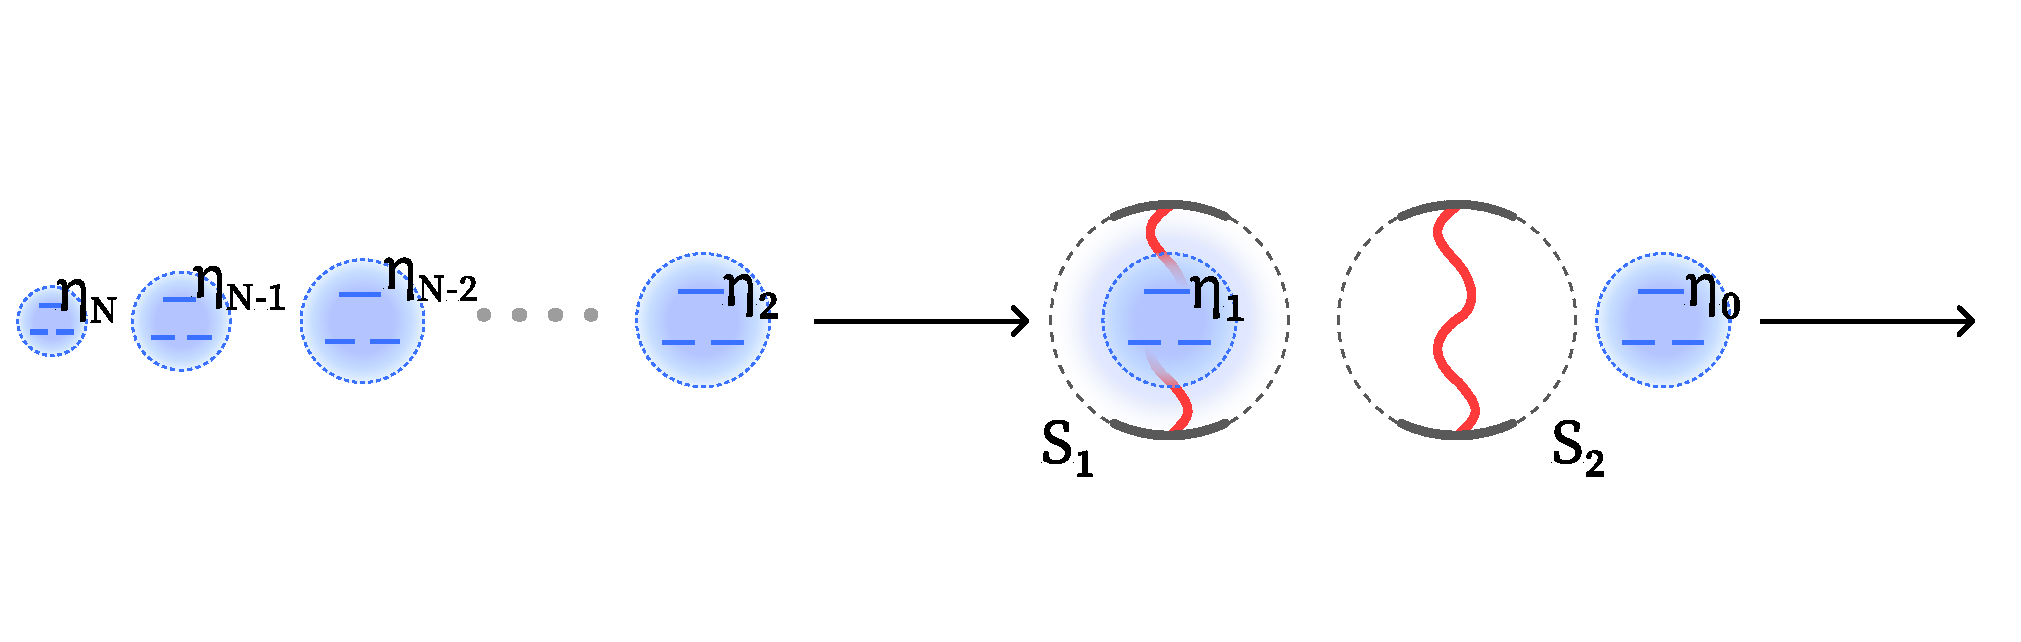
\includegraphics[width=0.9\textwidth]{images/phaseonium_horizontal.pdf}
\caption{ Standard collision model for a phaseonium bath interacting with a multipartite system. The system of interest is a cascade of two single-mode cavity fields $S_1$, $S_2$, which is described by a density operator $\rho$. The environment is made up of $N$ three-level atoms in lambda configuration, called phaseonium atoms, all prepared equally. These atoms play the role of ancillas and are described by a density operator $\eta_k$ ($k=0,\ldots, N$). Ancillas travel at speed $v$ and enter the cavities at a rate $r$. They interact with each cavity field for a time $\Delta t$. The speed and rate of phaseonium atoms is selected such that there is at most one ancilla in each cavity at a time.}
\label{fig:cascade-setup}
\end{figure*}

Each cavity is coupled to the environment via short-time interactions with ancilla systems pumped in the cavity itself. 
Every ancilla $\eta_k\,,k=0,\ldots,N$, is a three-level lambda system. Its states are denoted by $\ket{e}$, $\ket{g_1}$, and $\ket{g_2}$, where $\ket{e}$ represents the excited state while $\ket{g_1}$, $\ket{g_2}$ are two ground states. 
In this basis, the coherent ancilla state which defines the phaseonium \cite{scully_extracting-work_2002} can be represented by the density operator
\begin{equation}
\label{def:ancilla-state}
    \eta_k = 
\begin{pmatrix}
\begin{array}{ccc}
    \alpha^2 & 0 & 0
\\
    0 & \frac{\beta^2}{2} & \frac{\beta^2}{2} e^{-i \phi} 
\\[.3em]
    0 & \frac{\beta^2}{2}  e^{i \phi } & \frac{\beta^2}{2} \\
\end{array}
\end{pmatrix}
\,.\end{equation}
with the condition $\abs{\alpha}^2~=~1-\abs{\beta}^2$ to have a unitary trace.
One can thus write a simple free Hamiltonian $\hat{H}_\eta = \hbar\omega_\eta\ket{e}\bra{e}$ for the phaseonium.

We choose a resonant coupling with $\omega_c = \omega_\eta \equiv \omega$ and use the interaction picture to leave the free evolution of both cavity and bath out of the analysis.
So, indicating with $\Omega$ the coupling strength, the total system-environment Hamiltonian at the $k$-th collision is given by the interaction term
\begin{equation}\label{def:interaction}
    \hat{V}_k = \hbar\Omega\left[ \a(\dyad{e}{g_1}+\dyad{e}{g_2}) + \ad(\dyad{g_1}{e}+\dyad{g_2}{e}) \right] \,.
\end{equation}
\\

%%%%%%%%%%%%%%%%%%%%%%%%%%%%%%%%%%%%%%%%%%
\section{Results}

\subsection{One Cavity}
% ============================ %
% FULL-COHERENT PHASEONIUM
% ============================ %
What is the full dynamics of the system under the interaction with a full-coherent phaseonium $\rho_{n+1}=\Tr\left[U\rho\otimes\eta_{\text{full}}U^\dagger\right]$?

\begin{equation}
    \eta_{\text{full}} = \begin{pmatrix}
        \alpha^2 & \chi_{21} & \chi_{31} \\
        \bar{\chi}_{21} & \frac{\beta^2}{2} & \eta_{32} \\
        \bar{\chi}_{31} & \bar{\eta}_{32} & \frac{\beta^2}{2}  
    \end{pmatrix}
\end{equation}

% CALCULATIONS
%\renewenvironment{imported}
{
% Phaseonium coherences
\newcommand{\chidowntwo}{\bar{\chi}_{31}}
\newcommand{\chidownone}{\bar{\chi}_{21}}
\newcommand{\chiupone}{\chi_{21}}
\newcommand{\chiuptwo}{\chi_{31}}
\newcommand{\etadown}{\bar{\eta}_{32}}
\renewcommand{\etaup}{\eta_{32}}
\renewcommand{\a}{\alpha^2}
\renewcommand{\b}{\frac{\beta^2}{2}}
}
{}

\begin{imported}
The unitary evolution operator is defined as:
\begin{equation}
    e^{i\theta\hat{V}_n} = \begin{pmatrix}
        C & i\Sd & i\Sd \\
        i\S & \frac{\Cp+\idd}{2}& \frac{\Cp-\idd}{2} \\
        i\S & \frac{\Cp-\idd}{2} & \frac{\Cp+\idd}{2}
    \end{pmatrix}
\end{equation}

Tracing out ancilla's degrees of freedom, we have

\begin{align}
    &\rho_{n+1} =
    \left( \a\C\r + i\chidownone\Sd\r + i\chidowntwo\Sd\r \right)\C
    \\ +&
    \left(\etadown\frac{\Cp-\idd}{2}\r + \b\frac{\Cp+\idd}{2}\r +i\chiupone\S\r \right)\frac{\Cp+\idd}{2}
     +
    \left(\etaup\frac{\Cp-\idd}{2}\r + \b\frac{\Cp+\idd}{2}\r +i\chiuptwo\S\r \right)\frac{\Cp+\idd}{2}
    \\ +&
    \left( \b\frac{\Cp-\idd}{2}\r + \etaup\frac{\Cp+\idd}{2}\r + i\chiuptwo\S\r \right)\frac{\Cp-\idd}{2}
    +
    \left( \b\frac{\Cp-\idd}{2}\r + \etadown\frac{\Cp+\idd}{2}\r + i\chiupone\S\r \right)\frac{\Cp-\idd}{2}
    \\ -&
    i\left( \chidowntwo\frac{\Cp-\idd}{2}\r + \chidownone\frac{\Cp+\idd}{2}\r + i\a\S\r \right)\Sd 
    -
    i\left( \chidownone\frac{\Cp-\idd}{2}\r + \chidowntwo\frac{\Cp+\idd}{2}\r + i\a\S\r \right)\Sd 
    \\ -&
    i\left( \chiupone\C\r +i\b\Sd\r +i\etadown\Sd\r \right)\S
    -
    i\left( \chiuptwo\C\r +i\b\Sd\r +i\etaup\Sd\r \right)\S
\end{align}

and so
\begin{align}
    &\rho_{n+1} =
    \left( \a\C\r + i\chidownone\Sd\r + i\chidowntwo\Sd\r \right)\C
    \\ +&
    \frac{1}{2}\left(\etadown\frac{\Cp-\idd}{2}\r + \b\frac{\Cp+\idd}{2}\r +i\chiupone\S\r 
     +
    \etaup\frac{\Cp-\idd}{2}\r + \b\frac{\Cp+\idd}{2}\r +i\chiuptwo\S\r \right)\Cp
    \\ +&
    \frac{1}{2}\left(\etadown\frac{\Cp-\idd}{2}\r + \b\frac{\Cp+\idd}{2}\r +i\chiupone\S\r 
     +
    \etaup\frac{\Cp-\idd}{2}\r + \b\frac{\Cp+\idd}{2}\r +i\chiuptwo\S\r \right)\idd
    \\ +&
    \frac{1}{2}\left( \b\frac{\Cp-\idd}{2}\r + \etaup\frac{\Cp+\idd}{2}\r + i\chiuptwo\S\r
    +
    \b\frac{\Cp-\idd}{2}\r + \etadown\frac{\Cp+\idd}{2}\r + i\chiupone\S\r \right)\Cp
    \\ -&
    \frac{1}{2}\left( \b\frac{\Cp-\idd}{2}\r + \etaup\frac{\Cp+\idd}{2}\r + i\chiuptwo\S\r
    +
    \b\frac{\Cp-\idd}{2}\r + \etadown\frac{\Cp+\idd}{2}\r + i\chiupone\S\r \right)\idd
    \\ -&
    i\left( \chidowntwo\frac{\Cp-\idd}{2}\r + \chidownone\frac{\Cp+\idd}{2}\r + i\a\S\r 
    +
    \chidownone\frac{\Cp-\idd}{2}\r + \chidowntwo\frac{\Cp+\idd}{2}\r + i\a\S\r \right)\Sd 
    \\ -&
    i\left( \chiupone\C\r +i\b\Sd\r +i\etadown\Sd\r 
    +
    \chiuptwo\C\r +i\b\Sd\r +i\etaup\Sd\r \right)\S
\end{align}

\begin{align}
    &\rho_{n+1} =
    \left( \a\C\r + i\chidownone\Sd\r + i\chidowntwo\Sd\r \right)\C
    \\ +&
    \frac{1}{2}\left((\etadown+\etaup)\frac{\Cp-\idd}{2}\r + \beta^2\frac{\Cp+\idd}{2}\r +i(\chiupone+\chiuptwo)\S\r \right)\Cp
    \\ +&
    \frac{1}{2}\left((\etadown+\etaup)\frac{\Cp-\idd}{2}\r + \beta^2\frac{\Cp+\idd}{2}\r +i(\chiupone+\chiuptwo)\S\r \right)\idd
    \\ +&
    \frac{1}{2}\left( \beta^2\frac{\Cp-\idd}{2}\r + (\etadown+\etaup)\frac{\Cp+\idd}{2}\r +i(\chiupone+\chiuptwo)\S\r \right)\Cp
    \\ -&
    \frac{1}{2}\left( \beta^2\frac{\Cp-\idd}{2}\r + (\etadown+\etaup)\frac{\Cp+\idd}{2}\r +i(\chiupone+\chiuptwo)\S\r \right)\idd
    \\ -&
    i\left( (\chidowntwo+\chidownone)\frac{\Cp-\idd}{2}\r + (\chidownone+\chidowntwo)\frac{\Cp+\idd}{2}\r + 2i\a\S\r \right)\Sd 
    \\ -&
    i\left( \chiupone\C\r +i(\beta^2 + \etadown + \etaup)\Sd\r 
    +
    \chiuptwo\C\r \right)\S
\end{align}

\begin{align}
    &\rho_{n+1} =
    \left[ \a\C + i\chidownone\Sd + i\chidowntwo\Sd \right]\r\C
    \\ +&
    \frac{1}{2}\bigg[(\etadown+\etaup)\frac{\Cp-\idd}{2} + \beta^2\frac{\Cp+\idd}{2} +i(\chiupone+\chiuptwo)\S 
    \\ &+
    \beta^2\frac{\Cp-\idd}{2} + (\etadown+\etaup)\frac{\Cp+\idd}{2} +i(\chiupone+\chiuptwo)\S \bigg]\r\Cp
    \\ +&
    \frac{1}{2}\bigg[(\etadown+\etaup)\frac{\Cp-\idd}{2} + \beta^2\frac{\Cp+\idd}{2} +i(\chiupone+\chiuptwo)\S 
    \\ &-
    \beta^2\frac{\Cp-\idd}{2} - (\etadown+\etaup)\frac{\Cp+\idd}{2} -i(\chiupone+\chiuptwo)\S \bigg]\r\idd
    \\ -&
    i\left[ (\chidowntwo+\chidownone)\left(\frac{\Cp-\idd}{2} + \frac{\Cp+\idd}{2}\right) + 2i\a\S \right]\r\Sd 
    \\ -&
    i\left[ \chiupone\C +i(\beta^2 + \etadown + \etaup)\Sd + \chiuptwo\C \right]\r\S
\end{align}

\begin{align}
    &\rho_{n+1} =
    \left[ \a\C + i\chidownone\Sd + i\chidowntwo\Sd \right]\r\C
    \\ +&
    \frac{1}{2}\bigg[\frac{1}{2}\left((\etadown+\etaup) + \beta^2 + \beta^2 + (\etadown+\etaup)\right)\Cp + 2i(\chiupone+\chiuptwo)\S 
    \\ &+
    \frac{1}{2}\left((\etadown+\etaup) + \beta^2 - \beta^2 - (\etadown+\etaup)\right)\idd \bigg]\r\Cp
    \\ +&
    \frac{1}{2}\bigg[\frac{1}{2}\left((\etadown+\etaup)+\beta^2-\beta^2-(\etadown+\etaup)\right)\Cp
    \\ &+
    \frac{1}{2}\left(-(\etadown+\etaup)+\beta^2+\beta^2-(\etadown+\etaup)\right)\idd  \bigg]\r\idd
    \\ -&
    i\left[ (\chidowntwo+\chidownone)\Cp + 2i\a\S \right]\r\Sd 
    \\ -&
    i\left[ \chiupone\C +i(\beta^2 + \etadown + \etaup)\Sd + \chiuptwo\C \right]\r\S
\end{align}

\begin{align}
    &\rho_{n+1} =
    \left[ \a\C + i\chidownone\Sd + i\chidowntwo\Sd \right]\r\C
    \\ +&
    \frac{1}{2}\bigg[\left(\beta^2 + \etadown+\etaup\right)\Cp + 2i(\chiupone+\chiuptwo)\S 
    \bigg]\r\Cp
    \\ +&
    \frac{1}{2}\bigg[\left(\beta^2-\etadown-\etaup\right)\idd  \bigg]\r\idd
    \\ -&
    i\left[ (\chidowntwo+\chidownone)\Cp + 2i\a\S \right]\r\Sd 
    \\ -&
    i\left[ \chiupone\C +i(\beta^2 + \etadown + \etaup)\Sd + \chiuptwo\C \right]\r\S
\end{align}

Now we call $B(\phi)\equiv(\beta^2+\etaup+\etadown)$ and $\bar{B}(\phi)\equiv(\beta^2-\etaup-\etadown)$:

\begin{align}
    \rho_{n+1} =&
    \a\C\r\C 
    +\frac{1}{2}B(\phi)\Cp\r\Cp
    +B(\phi)\Sd\r\S 
    +2\a\S\r\Sd 
    +\frac{1}{2}\bar{B}(\phi)\idd\r\idd
    \\
    &+i(\chidownone+\chidowntwo)(\Sd\r\C - \Cp\r\Sd)
    +i(\chiupone+\chiuptwo)(\S\r\Cp - \C\r\S)
\end{align}

With our previous notation $\etaup = \b e^{-i\phi}$ and $\etadown = \b e^{i\phi}$
\begin{align}
    B(\phi) =& \beta^2+\etaup+\etadown = \beta^2 + \b (e^{-i\phi} + e^{i\phi}) \\
    &\,= \beta^2 (1 + 1/2(\cos\phi -i\sin\phi + \cos\phi +i\sin\phi)) = \beta^2(1+\cos\phi) 
    \\
    \bar{B}(\phi) =& \beta^2-\etaup-\etadown = \beta^2 - \b (e^{-i\phi} + e^{i\phi}) \\
    &\,= \beta^2 (1 - 1/2(\cos\phi -i\sin\phi + \cos\phi +i\sin\phi)) = \beta^2(1 - \cos\phi) 
\end{align}
then $2\alpha^2 = \gamma_\alpha$ and $\beta^2(1+\cos\phi) = \gamma_\beta$.
\\[10pt]


% This is given by Kraus Operators:
%\begin{align}
%    \hat{E}_0 =& \sqrt{\frac{\beta^2}{2}(1-\cos\phi)}\idd \,, \\
%    \hat{E}_1 =& \frac{\sqrt{\ga}}{2}\C \,, \\
%    \hat{E}_2 =& \sqrt{\gamma_\alpha}\Sd \,, \\
%    \hat{E}_3 =& \sqrt{\frac{\gamma_\beta}{2}}\Cp \,, \\
%    \hat{E}_4 =& \sqrt{\gamma_\beta}\S \,,\\
%\end{align}
\end{imported}
\vspace{5pt}

Eventually we find the discrete Master Equation
\begin{equation}\label{eq:full-coherent-map}
\begin{split}
    \rho_{n+1} =&
    \alpha^2\C\rho_n\C 
    +2\alpha^2\S\rho_n\Sd 
    +\frac{\beta^2}{2}(1+\cos\phi)\Cp\rho_n\Cp
    +\beta^2(1+\cos\phi)\Sd\rho_n\S 
    +\frac{\beta^2}{2}(1 - \cos\phi)\idd\rho_n\idd
    \\
    &+i(\bar{\chi}_{21}+\bar{\chi}_{31})(\Sd\rho_n\C - \Cp\rho_n\Sd)
    +i(\chi_{21}+\chi_{31})(\S\rho_n\Cp - \C\rho_n\S)
\end{split}
\end{equation}
where the first line is equal to our known Kraus map and the second line is a work term, with an effective Hamiltonian $H_{\text{work}}$.


% ========================== %
\subsubsection{Continuous Times}
% ========================== %
For short-time approximation, photonic operators in Eq.~\ref{eq:full-coherent-map} become
\begin{equation}\label{eq:short-time-approx}
    %&\equiv \cos(\theta\sqrt{2aa^\dagger}) \rightarrow
    C=\mathbb{I} - \theta^2aa^\dagger \qquad
    %\cos(\theta\sqrt{2a^\dagger a}) 
    C'= \mathbb{I} - \theta^2a^\dagger a \qquad
    % a^\dagger \frac{\sin(\theta\sqrt{2aa^\dagger})}{\sqrt{2aa^\dagger}} 
    S = \theta a^\dagger 
\end{equation}

% CALCULATIONS
%\renewenvironment{imported}{
% Local new commands here
% \newcommand{}{}
}
{}


Neglecting terms of the order $\Delta t^3$ ($\theta^3$) and higher we have:

\begin{align}
    \rho_{n+1} =&
    \alpha^2\left(\r - \tt\r\a\ad - \tt\a\ad\r \right)
    +2\alpha^2\left( \tt\ad\r\a \right)\\
    &+\frac{\beta^2}{2}(1+\cos\phi)\left( \r -\tt\r\ad\a -\tt\ad\a\r \right)   +\beta^2(1+\cos\phi)\left( \tt\a\r\ad \right) \\
    &+i(\bar{\chi}_{21}+\bar{\chi}_{31})(\theta\a\r\idd - \theta\idd\r\a) \\
    &+i(\chi_{21}+\chi_{31})(\theta\ad\r\idd - \theta\idd\r\ad) \\
    &+\frac{\beta^2}{2}(1 - \cos\phi)\r
\end{align}
and so
\begin{align}
    \rho_{n+1} =&
    \alpha^2\left( - \tt\r\a\ad - \tt\a\ad\r 
    +2\tt\ad\r\a \right) +\alpha^2\r \\
    &+\frac{\beta^2}{2}(1+\cos\phi)\left( -\tt\r\ad\a -\tt\ad\a\r + 2\tt\a\r\ad \right) +\frac{\beta^2}{2}(1+\cos\phi)\r\\
    &+i\theta(\bar{\chi}_{21}+\bar{\chi}_{31})(\a\r - \r\a) \\
    &+i\theta(\chi_{21}+\chi_{31})(\ad\r - \r\ad) \\
    &+\frac{\beta^2}{2}(1 - \cos\phi)\r
\end{align}
and this is
\begin{align}
    \rho_{n+1} =&
    2\alpha^2\tt\left(\ad\r\a -\frac{1}{2}\acomm{\a\ad}{\r} \right) \\
    &+\beta^2(1+\cos\phi)\tt\left(\a\r\ad -\frac{1}{2}\acomm{\ad\a}{\r} \right) \\
    &+i\theta\comm{(\bar{\chi}_{21}+\bar{\chi}_{31})\a + (\chi_{21}+\chi_{31})\ad}{\r} \\
    &+\left( \alpha^2 +\frac{\beta^2}{2}(1+\cos\phi) + \frac{\beta^2}{2}(1 - \cos\phi) \right)\r
\end{align}

The final form of the master equation is:
\begin{equation}
\begin{split}
    \frac{\rho_{n+1} - \rho_n}{\Delta t} =
    +&i\comm{\hbar\Omega H_{\text{work}}}{\r} \\
    +&\ga(\hbar\Omega)^2\Delta t\left(\ad\rho_n\a -\frac{1}{2}\acomm{\a\ad}{\rho_n} \right)
    +\gb(\hbar\Omega)^2\Delta t\left(\a\rho_n\ad -\frac{1}{2}\acomm{\ad\a}{\rho_n} \right) 
\end{split}
\end{equation}
with $H_{\text{work}}\equiv(\bar{\chi}_{21}+\bar{\chi}_{31})\a + (\chi_{21}+\chi_{31})\ad$.

\subsection{Two Cavities}
\renewcommand{\b}{\hat{b}}
We now derive the master equation describing the dynamics of the two cavities in the case in which are present coherence also between the excited and the two ground states of the phaseonium bath. 


In this case $\rho_n \in \mathcal{H}_1\otimes\mathcal{H}_2$ and $\sigma_n=\rho_n\otimes\eta$, so the evolution is described by
\begin{equation}
\sigma_{n+1}=U_2 U_1\sigma_n U^\dagger_1 U^\dagger_2
\end{equation}

Taking the continuous limit, i.e. taking $U_i$ up to the second order, and denoting $\a$ ( $\ad$ ) and $\hat{b}$ ($\bd$) as the annihilation (creation) operators for the first  and second cavity respectively,

\begin{multline}
\sigma_{n+1}=(\mathbb{I}-i\theta V_2-\frac{\theta^2}{2} V^2_2)(\mathbb{I}-i\theta V_1-\frac{\theta^2}{2} V^2_1)\sigma_n(\mathbb{I}+i\theta V_1-\frac{\theta^2}{2} V^2_1)(\mathbb{I}+i\theta V_2-\frac{\theta^2}{2} V^2_2)=\\
=(\mathbb{I}-i\theta V_2-i\theta V_1-\frac{\theta^2}{2} V^2_2-\frac{\theta^2}{2} V^2_1-\theta^2V_2V_1)\sigma_n(\mathbb{I}+i\theta V_2+i\theta V_1-\frac{\theta^2}{2} V^2_2-\frac{\theta^2}{2} V^2_1-\theta^2V_1V_2)=\\
=\sigma_n-i\theta[V_2,\sigma_n]-i\theta[V_1,\sigma_n]+\theta^2V_1\sigma_nV_2+\theta^2V_2\sigma_nV_1+\\+\theta^2(V_1\sigma_nV_1-\frac{1}{2}[V^2_1,\sigma_n]_+)+\theta^2(V_2\sigma_nV_2-\frac{1}{2}[V^2_2,\sigma_n]_+)-\theta^2V_2V_1\sigma_n-\theta^2V_1V_2\sigma_n
\end{multline}

Taking the difference between the ($n+1$)-th step and the n-th step, dividing by $\theta$ and tracing out the degrees of freedom one obtains 

\begin{align}\label{def:lindbladian-evolution-two-cavities}
    \frac{d\rho(t)}{d t}
    %= &\mathcal{L}\hat{\rho}(t)\\
    = -i[\hat{H}_\text{eff},\rho] +  \gamma'_\alpha \,\mathcal{D}[\hat{a}^\dagger{+}\hat{b}^\dagger]\,\hat{\rho}(t)+\gamma'_\beta \,\mathcal{D}[\hat{a}{+}\hat{b}]\,\hat{\rho}(t)
\end{align}

where $\hat{H}_\text{eff}=i(\gamma'_\beta-\gamma'_\alpha)(\a\b-\bd\a)/2+((\bar{\chi}_{21}+\bar{\chi}_{31})(\a+\b)+(\chi_{21}+\chi_{31})(\ad+\bd) )$

\subsection{Making things useful: Reciprocating Quantum Engines}
To exploit the properties of the quantum world one has to use non-thermal systems, where temperature may not be well defined.
To extract work from those systems is possible with the same methods of classical quantum thermodynamics, but it is worth calling those machines Quantum Engines (QEs) rather than Quantum Thermal Engines (QTEs).
\textcolor{red}{For simplicity, our QE will perform an Otto cycle, where \textbf{work} and \textbf{heat} are decoupled in different strokes.}
The most simple cycle to perform with a QE is the Otto cycle, where \textbf{work} and \textbf{heat} are decoupled in different strokes.

The Otto cycle works like this:
\begin{itemize}
    \item (A) System starts in A at temperature $T_A$ and entropy $S_A$
    \begin{itemize}
    {\item (1) \textbf{Isochore Stroke:} Going from A to B in stroke 1 the system absorbs heat from a \emph{ground-coherent} phaseonium at tempreture $T_\eta$}
    \end{itemize}
    \item (B) System is in B at temperature $T_B > T_A$ and entropy $S_B > S_A$, where $T_B \equiv T_\phi$ is dependent upon phaseonium coherences
    \begin{itemize}
    {\item (2) \textbf{Adiabatic Stroke:} Going from B to C in stroke 2 the system do positive work on the environment}
    \end{itemize}
    \item (C) System is in C at temperature $T_C < T_B$ with the same entropy as B, $S_C = S_B = S_h$
    \begin{itemize}
    {\item (3) \textbf{Isochore Stroke:} Going from C to D in stroke 3 the system relase heat to a  \emph{thermal} phaseonium at temperature $T_\eta$}
    \end{itemize}
    \item (D) System is in D at temperature $T_D < T_C < T_A$ and entropy $S_D = S_A = S_l$, where $T_D = T_\eta$
    \begin{itemize}
    {\item (4) \textbf{Adiabatic Stroke:} Going from D back to A in stroke 4 work is done on the system by \emph{upper-coherent} phaseonium at temperature $T_\eta$ }
    \end{itemize}
\end{itemize} 

In our case \emph{we cannot} perform such a cycle using Phaseonium. 
In fact, Eq.~\ref{eq:full-coherent-map} and Eq.~\ref{def:lindbladian-evolution-two-cavities} present dissipative terms which cannot be removed.
Thus, we cannot perform the adiabatic strokes 2 and 3.
Instead, we can implement two isobaric strokes guided by phaseonium atoms, where the ``pressure'' under consideration is the \textbf{radiation pressure} $p$ of the electromagnetic field on one of the mirrors.
As explained in Ref.~\cite{tejero_atom-doped_2024}, we can define the Radiation Pressure Operator as
\begin{equation}\label{def:radiation-pressure}
    \pi(t) \equiv \frac{\omega}{2V(t)}\left( \ad\a + \a\ad - \a\a e^{-i2\omega t} - \ad\ad e^{i2\omega t} \right) \,,
\end{equation}
so that at every time $t$ we can measure the pressure $p(t)$ as the expectation value $\expval{\pi(t)}=\Tr\left[\pi(t)\rho(t)\right]$, or, in our step-wise dynamics: $p_n = \Tr\left[\pi_n\rho_n\right]$.
For an isobaric stroke, we have $\Delta p_n = 0$. This equation should give a condition on $V(t)$ which should increase or decrease accordingly. In turn, the variable size of the cavity will make the system's Hamiltonian varying in time due to the frequency-length relation $\omega \propto 1/L(t)$.

We can go further giving a general expression for the evolution of \emph{pressure} in a cavity under the action of Phaseonium.

\subsubsection{Pressure}
We that an operator, in this case $\hat{\pi}$ evolves at step $k$ as
\begin{align}
    \Delta\expval{\hat{\pi}}_k &= \Tr\left\{\hat{\pi}\rho_{k+1}\right\} - \Tr\left\{\hat{\pi}\rho_{k}\right\} \\
    =& \Tr\left\{\hat{\pi}\left(\sum_{i=0}^4\hat{E_i}\rho_k\hat{E_i}^\dagger - \rho_k\right)\right\} = \Tr\left\{\left(\sum_{i=0}^4\hat{E_i}^\dagger\hat{\pi}\hat{E_i} - \hat{\pi}\right) \rho_k\right\} \\
    =& \Tr\left\{\Delta\hat{\pi}\,\rho_{k}\right\}\;.
\end{align}
Thus, we can define the operator Master Equation
\begin{equation}
    \Delta\expval{\hat{\pi}}_k = \sum_{i=1}^4\expval{\widetilde{\mathcal{D}}\left[\hat{E}_i\right]\hat{\pi}}
\end{equation}
and $\widetilde{\mathcal{D}}[\hat E]\hat{\pi}=\hat E^\dagger\hat{\pi}\hat E-1/2\{\hat E^\dagger\hat E,\hat{\pi}\}$.

In the fast-interaction approximation $\Delta t\ll1$, the average pressure at step $k$ is given by the expectation value
\begin{align}
    \Delta p_k = \tt \big \langle&\\
    &\quad\ga\left[\a\hat{\pi}\ad - \frac{1}{2}\left(\a\ad\hat\pi+\hat\pi\a\ad\right) \right] +\\
    &\quad\gb\left[\ad\hat{\pi}\a - \frac{1}{2}\left(\ad\a\hat\pi+\hat\pi\ad\a\right) \right] \\
    \big\rangle
\end{align}

% ========================== %
\newpage
\subsection{Ancilla Evolution}
% ========================== %
If we are to use phaseonium atoms as fuel for multiple cavities, we must consider the evolution of ancillas after every collision with the cavities.
This is a collision model problem in which this time one phaseonium atom is the system and cavities are the ancillas, as depicted in Fig.~\ref{fig:phaseonium-collisional}.
We consider a beam of $N + 1$ phaseonium atoms passing through $M + 1$ cavities, interacting for a time $\Delta t$. 
Each atom $\eta_k$ will evolve from step $0$ to step $M$ at discrete time steps, colliding with all the cavities from $0$ to $M$, and the notation $\eta_k(n)$ as well as $\rho_k(n)$ will refer to the density matrix of the $k$th phaseonium atom or cavity at evolutionary step $n$.
The cavities seen by this atom will have already collided with all preceding $k$ atoms, so they already evolved from step $0$ to step $k$.
We can choose an equal initial state for all the cavities, $\rho_0(0)=\rho_1(0)=\cdots=\rho_M(0)$, so that $\eta_0$ interacts with equal ancillas.
However, this first interaction will have different effects on the cavities, due to the evolution of $\eta_0$ from one step to the other: each cavity will be in a state $\rho_0(1)\neq\rho_1(1)\neq\cdots\neq\rho_M(1)$ after the interaction with $\eta_0$.

\begin{figure*}
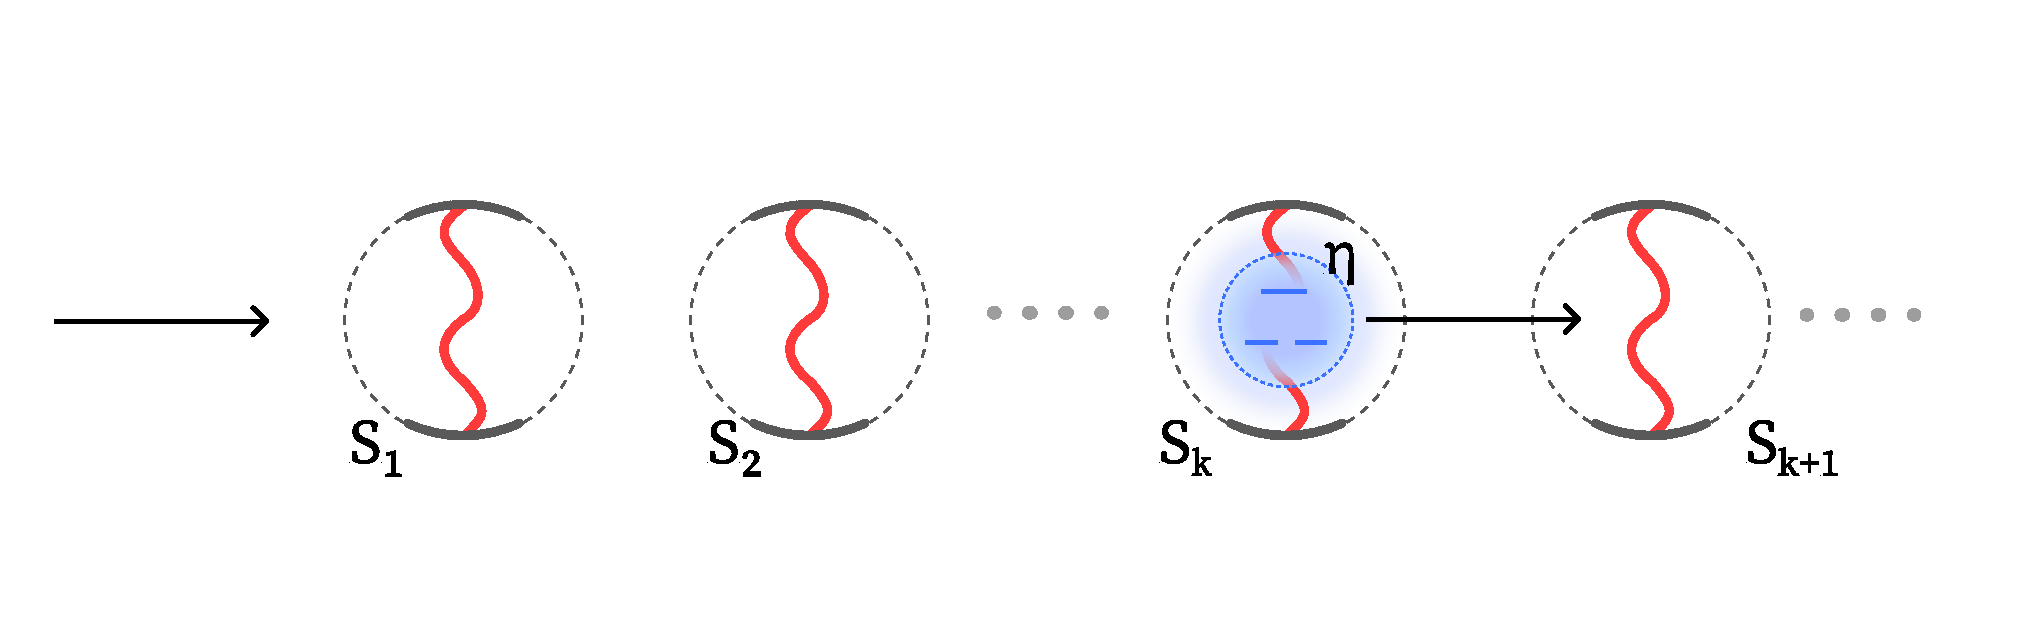
\includegraphics[width=0.9\textwidth]{images/phaseonium2_horizontal.pdf}
\caption{ Collision model for a phaseonium atom interacting with a cascade of cavity fields. For consistency we call the cavities $S_k$, ($k=0,\ldots, N$), although they are treated as ancillas and not systems. Phaseonium atom is described by a density operator $\eta$. In the reference frame of the phaseonium, cavities travel at speed $v$ and collide with the atom at a rate $r$. The atom interact with each cavity field for a time $\Delta t$. The speed and rate of phaseonium atoms is selected such that there is at most one atom in each cavity at a time.}
\label{fig:phaseonium-collisional}
\end{figure*}
%CALCULATIONS
\renewenvironment{imported}{
    % Local new commands here
    % \newcommand{}{}
    \newcommand{\s}{\hat{\sigma}}
}{}

\begin{imported}

Using the standard collision model techniques (cfr. \cite{ciccarello_quantum-collision_2022}), we can cast the interaction term in Eq.~\ref{def:interaction} as $\hbar\Omega(A_+B_+ + A_-B_-)$, where
\begin{equation}
    A_+ = \ad,\;\,A_-=\a,\;\,B_+=\s_1^-+\s_2^-\,,\;\,B_-=\s_1^++\s_2^+\,.
\end{equation}
Next, we focus only on the first atom reaching the cavities, $\eta_0$, and its evolution from $\eta_0(0)$ to $\eta_0(M)$.
Eventually we will set $M=2$ as in our case.
The joint system at evolutionary step $n$ will be $\sigma_n = \eta_0(n)\otimes\rho_{n}(0)$.
In fact, every cavity from $\rho_0$ to $\rho_M$ will not have evolved, so that they are all in evolutionary step $0$.
In Interaction picture the joint system evolves according to $\sigma_{n+1}=\exp{-i\Delta tV_n}\,\sigma_n\exp{i\Delta tV_n}$.
Expanding the exponential to second order in $\Delta t$ we have
\begin{equation}
    \Delta\sigma_{n+1} = -i\comm{H_0+V_n}{\sigma_n}+\Delta t^2\left( V_n\sigma_nV_n-\frac{1}{2}\acomm{V_n^2}{\sigma_n}\right)
\end{equation}
Dividing by $\Delta t$ and tracing off the ancilla (cavity) state $\rho_n(0)$ we can write directly the Master Equation for the evolution of the phaseonium state from $\eta_0(n)$ to $\eta_0(n+1)$ as
\begin{align}
    \frac{\Delta\eta_0(n+1)}{\Delta t} =& -i\comm{\hat{H}_S+\sum_\nu g_\nu\ev{A_\nu}B_\nu}{\eta_0(n)} \\
    &+\sum_{\nu\mu}g_\nu g_\mu\Delta t\ev{A_\mu A_\nu}\left( B_\nu\eta_0(n)B_\mu-\frac{1}{2}\acomm{B_\mu B_\nu}{\eta_0(n)} \right),
\end{align}
with $\nu,\mu = +,-$.
The Master Equation requires the calculation of expectation values with respect to the cavity density matrix $\rho_n(0)$. If we choose a common initial state $\rho_0\equiv\rho_n(0),\,n=0,\ldots M$, we can define
\begin{align}
    \ev{A_+} &= \Tr{\ad\rho_0}\equiv A^+_0,\\
    \ev{A_-} &= \Tr{\a\rho_0}\equiv A^-_0,\\
    \ev{A_+ A_+} &= \Tr{\ad\ad\rho_0}\equiv A^{++}_0,\\
    \ev{A_- A_-} &= \Tr{\a\a\rho_0}\equiv A^{--}_0,\\
    \ev{A_+ A_-} &= \Tr{\ad\a\rho_0}\equiv P_0,\\
    \ev{A_- A_+} &= \Tr{\a\ad\rho_0}\equiv P_0 + 1.\\
\end{align}


\end{imported}


 



%%%%%%%%%%%%%%%%%%%%%%%%%%%%%%%%%%%%%%%%%%
\section{Discussion}

Authors should discuss the results and how they can be interpreted from the perspective of previous studies and of the working hypotheses. The findings and their implications should be discussed in the broadest context possible. Future research directions may also be highlighted.

%%%%%%%%%%%%%%%%%%%%%%%%%%%%%%%%%%%%%%%%%%
\section{Conclusions}

This section is not mandatory, but can be added to the manuscript if the discussion is unusually long or complex.


%%%%%%%%%%%%%%%%%%%%%%%%%%%%%%%%%%%%%%%%%%
\vspace{6pt} 


\section[\appendixname~\thesection]{}
All appendix sections must be cited in the main text. In the appendices, Figures, Tables, etc. should be labeled, starting with ``A''---e.g., Figure A1, Figure A2, etc.


\bibliographystyle{abbrv}
\bibliography{thermodynamics}

\end{document}

